\documentclass[a4paper,12pt]{article}
\usepackage[utf8]{inputenc}
\usepackage[spanish]{babel}

% APA con biblatex
\usepackage[backend=biber,style=apa]{biblatex}
\DeclareLanguageMapping{spanish}{spanish-apa}
\addbibresource{Referencias.bib}

% Otros paquetes
\usepackage{graphicx}
\usepackage{float}
\usepackage{caption}
\usepackage{setspace}
\usepackage{fancyhdr}
\usepackage{geometry}
\geometry{left=3cm,right=3cm,top=2.5cm,bottom=2.5cm}

\setlength\bibitemsep{1.5\baselineskip}
\setlength{\parindent}{0pt}
\setlength{\parskip}{0.8em}

\pagestyle{fancy}
\fancyhf{}
\rhead{\thepage}
\lhead{\textit{Anexos}}

\begin{document}

\begin{center}
    \Large \textbf{Anexos}
\end{center}

\renewcommand{\thefigure}{A\arabic{figure}}
\setcounter{figure}{0}

% -------------------------------------------------------------------
\section{Líneas de continuidad y posibilidades de desarrollo futuro}
% -------------------------------------------------------------------

El presente anexo reúne las principales líneas de continuidad identificadas durante el desarrollo del modelo termodinámico del motor rotativo de seis tiempos. Estas propuestas no formaron parte del alcance central del estudio, pero representan rutas claras para ampliar la investigación. Su objetivo es servir como guía para quienes deseen extender, complementar o validar el modelo planteado en este trabajo, abarcando aspectos geométricos, termodinámicos, mecánicos y de manufacturabilidad que pueden convertir esta arquitectura en una alternativa viable para estudios futuros.

% -------------------------------------------------------------------
\section{Posibilidades derivadas de la geometría rotor–estator}
% -------------------------------------------------------------------

La configuración geométrica del motor permite múltiples combinaciones de ciclos según el número de lóbulos del estator y el número de puntas del rotor. Cada conjunto ofrece modos de operación únicos y abre la posibilidad de concebir motores multifrecuencia, híbridos o de alta densidad de potencia.

\subsection{Configuración 3--4 (estator de tres lóbulos, rotor de cuatro puntas)}

La geometría 3--4 permite una flexibilidad que no se observa en motores rotativos convencionales. Esta configuración puede operar simultáneamente como un motor de cuatro tiempos y un motor de dos tiempos, ya que una cavidad puede ejecutar un ciclo Otto completo mientras otra, por su posición angular, puede completar un ciclo de dos tiempos dentro de la misma revolución. Asimismo, esta arquitectura permite desarrollar tres ciclos consecutivos de dos tiempos en una sola vuelta del rotor, lo que aumenta la frecuencia de combustión y la potencia específica. También resulta posible asignar diferentes ciclos a distintas cavidades, generando configuraciones híbridas como 2T--4T--2T, lo que habilita evaluar cambios en eficiencia térmica, suavidad del torque y comportamiento dinámico general del motor.

\begin{figure}[H]
    \centering
    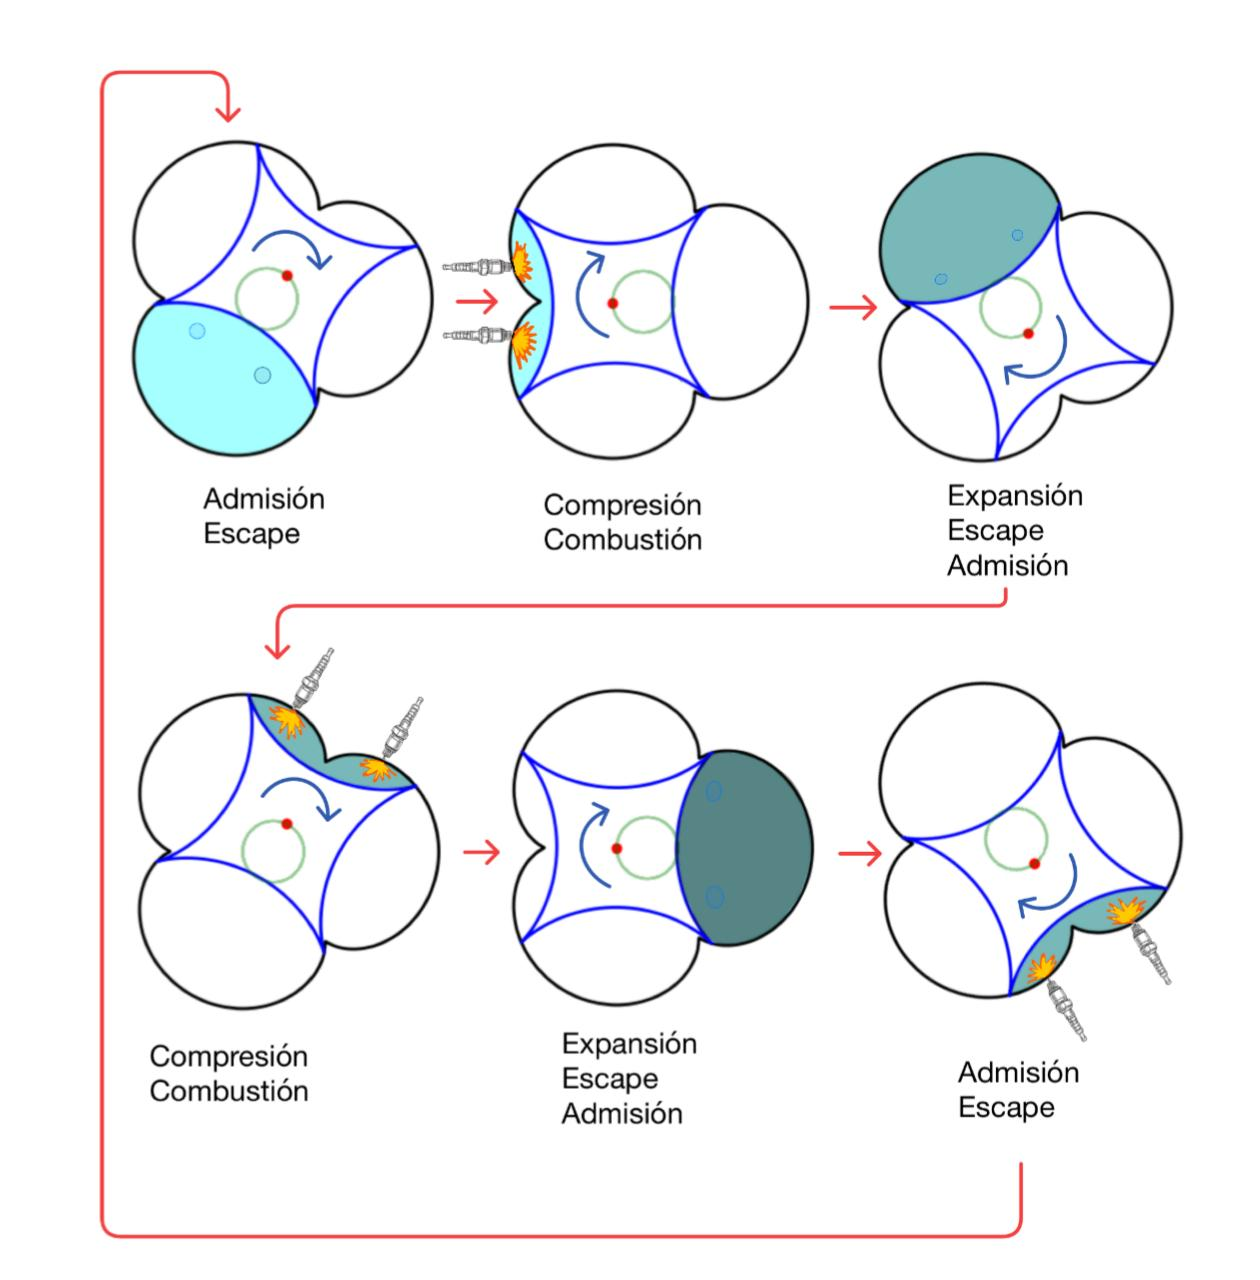
\includegraphics[width=0.7\textwidth]{3L4P_2T.jpg} % Cambia por el nombre real del archivo
    \caption{Secuencia de funcionamiento de la configuración con estator de tres lóbulos y rotor de cuatro puntas operando como tres motores de dos tiempos por revolución. Cada cavidad completa de manera independiente las etapas de compresión--combustión y expansión--escape, generando tres impulsos de trabajo en un giro del rotor.}
    \label{fig:3x2T}
\end{figure}

\begin{figure}[H]
    \centering
    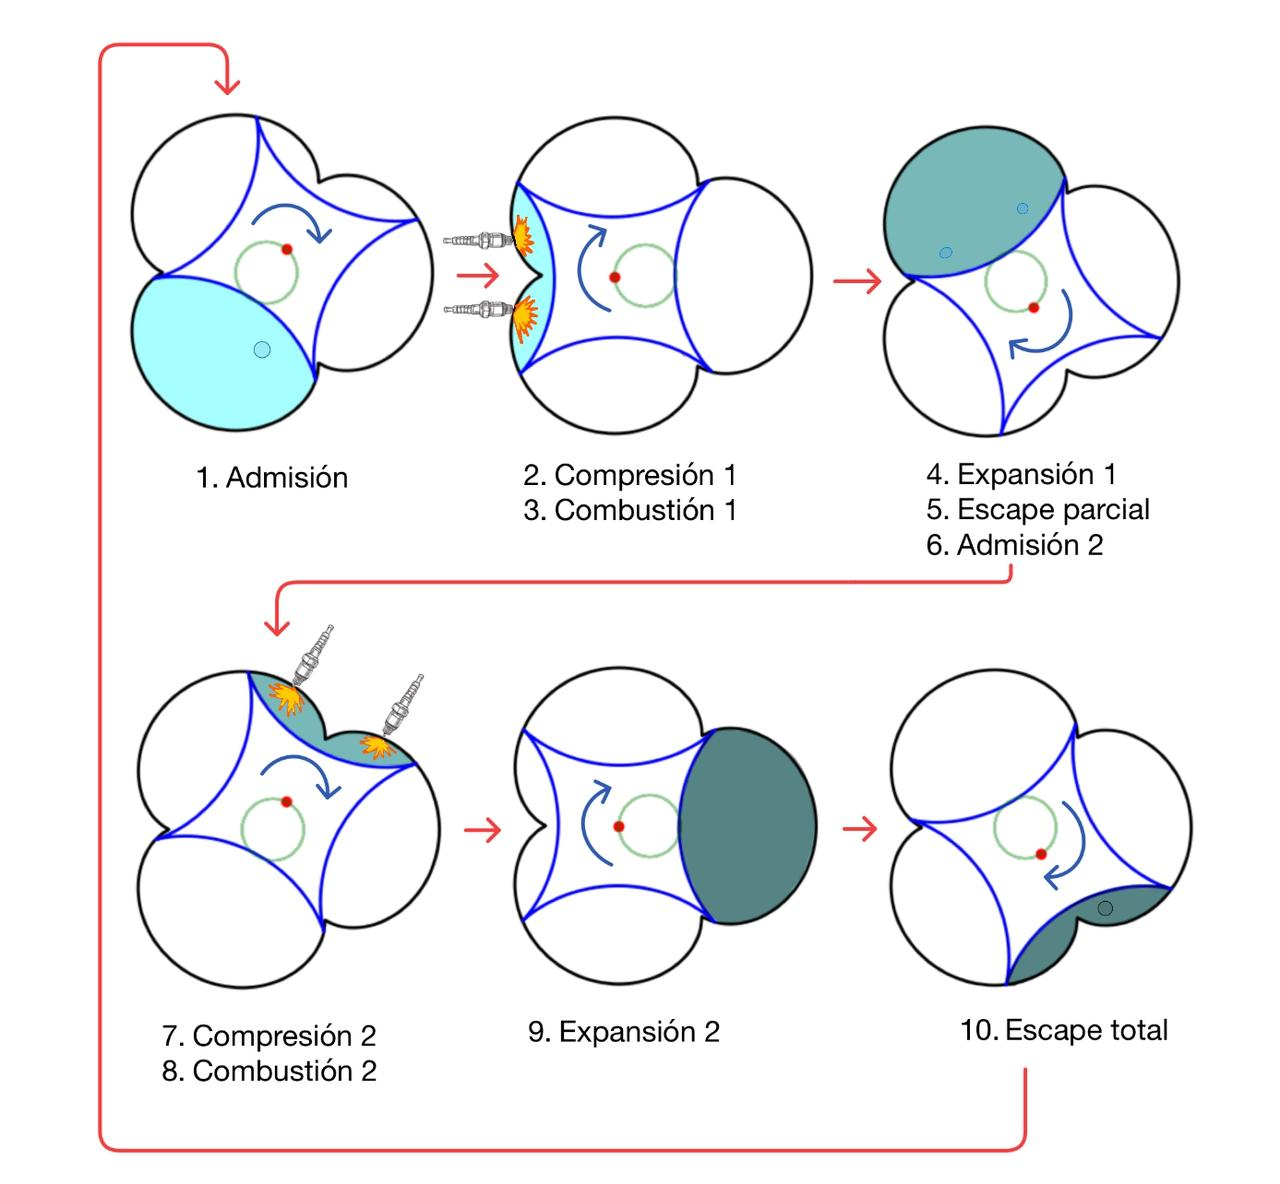
\includegraphics[width=0.7\textwidth]{3L4P_4T.jpg} % Cambia por el nombre real del archivo
    \caption{Secuencia de funcionamiento híbrido en la configuración de tres lóbulos y cuatro puntas. La cavidad ejecuta inicialmente un ciclo de dos tiempos (admisión, compresión--combustión, expansión y escape parcial) seguido por un ciclo de cuatro tiempos (admisión, compresión--combustión, expansión y escape total), permitiendo un ciclo extendido 2T--4T dentro de una misma revolución del rotor.}
    \label{fig:2T4T}
\end{figure}



\subsection{Configuración 4--5 (estator de cuatro lóbulos, rotor de cinco puntas)}

La configuración 4--5 incrementa el número de cavidades y, con ello, la capacidad de generar pulsos de potencia por revolución. En este conjunto, cada cavidad puede funcionar como un motor de dos tiempos, produciendo hasta cuatro combustiones dentro de una misma vuelta. Alternativamente, la presencia de dos puntos de volumen mínimo permite que el sistema opere como dos motores de cuatro tiempos superpuestos, duplicando la frecuencia de combustión con respecto a un motor Wankel tradicional. También es posible desarrollar modos escalonados en los que cada cavidad ejecute un tiempo distinto, lo que favorece estudios sobre motores multifase y sobre estrategias para suavizar el torque o aumentar la presión media efectiva.

\begin{figure}[H]
    \centering
    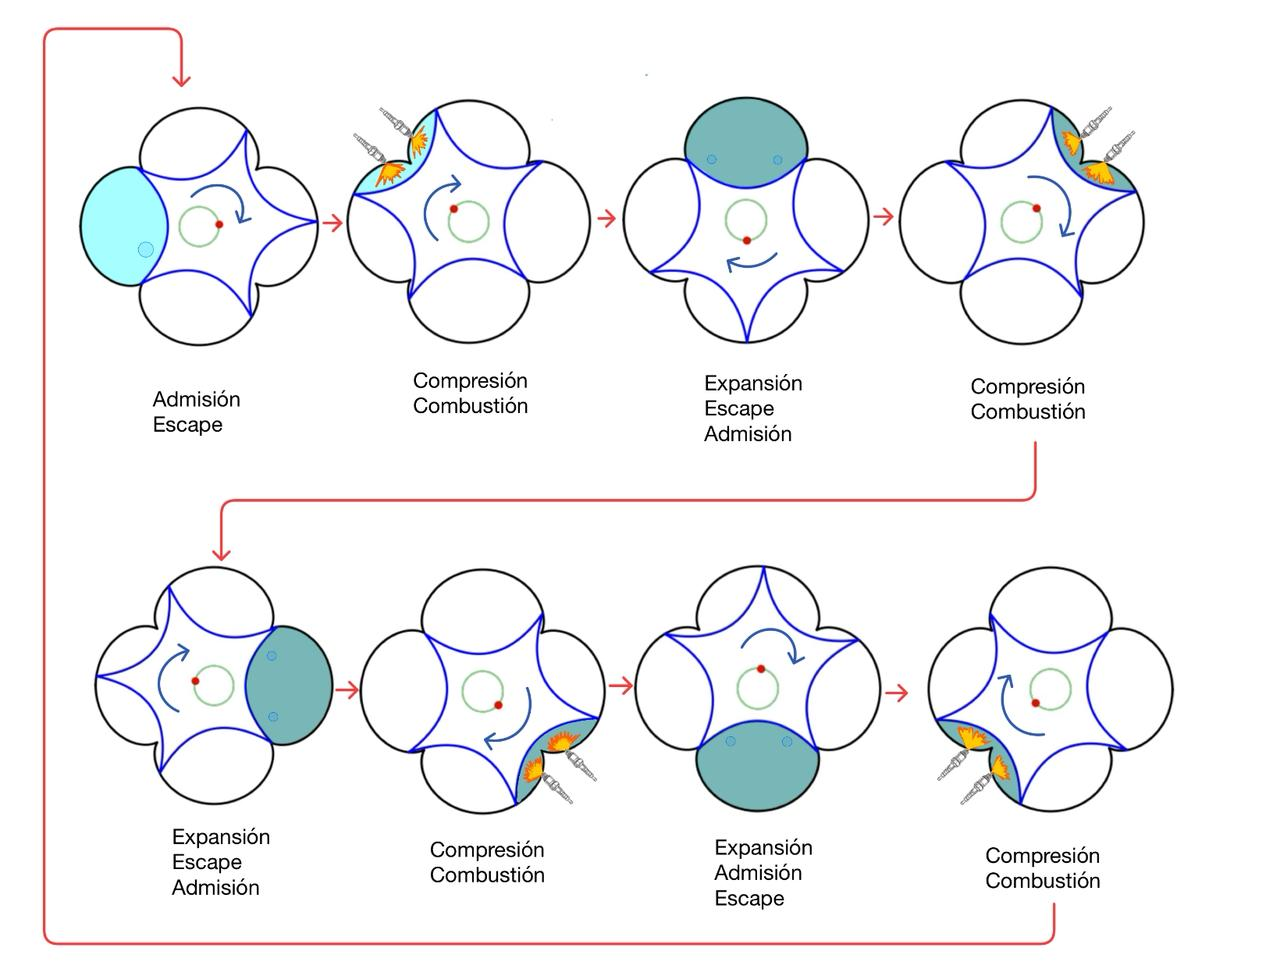
\includegraphics[width=0.7\textwidth]{4L5P_2T.jpg} % Cambia el nombre por el archivo real
    \caption{Secuencia de operación del conjunto de cuatro lóbulos y cinco puntas funcionando como cuatro motores de dos tiempos en una misma revolución. Cada cavidad completa un ciclo de compresión--combustión y expansión--escape al alcanzar su volumen mínimo, produciendo cuatro impulsos de trabajo por vuelta.}
    \label{fig:4x2T}
\end{figure}

\begin{figure}[H]
    \centering
    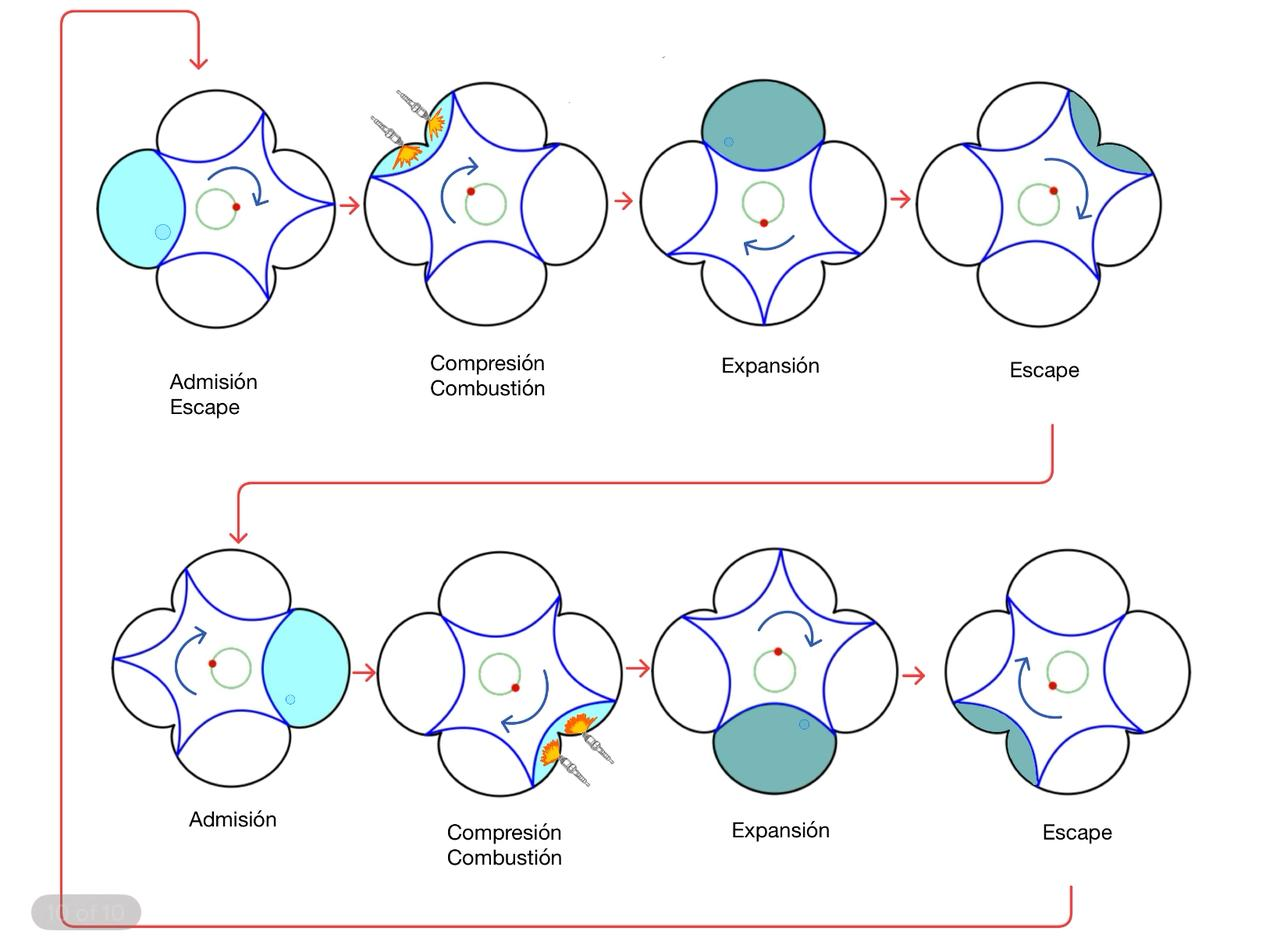
\includegraphics[width=0.7\textwidth]{4L5P_4T.jpg} % Cambia por el nombre real del archivo
    \caption{Secuencia de operación del conjunto con cuatro lóbulos y cinco puntas funcionando como dos ciclos completos de cuatro tiempos por revolución. Cada zona de volumen mínimo permite ejecutar un ciclo Otto independiente, generando dos procesos de admisión, compresión--combustión, expansión y escape en un giro del rotor.}
    \label{fig:4lob2x4T}
\end{figure}



% -------------------------------------------------------------------
\section{Mejoras funcionales aplicables al ciclo}
% -------------------------------------------------------------------

Una de las líneas de continuidad más interesantes consiste en incorporar un sistema de válvulas de apertura variable. Al modificar dinámicamente el tiempo de apertura, sería posible optimizar la admisión de aire, mejorar el barrido de gases y regular la cantidad de hidrocarburos no quemados presentes en el escape. Este sistema permitiría adaptar el funcionamiento del motor a diferentes condiciones de carga y velocidad sin alterar la geometría básica del conjunto rotor–estator.

Otra alternativa consiste en habilitar una doble combustión dentro de la misma cavidad. Este proceso se lograría permitiendo la expulsión parcial de hidrocarburos no quemados tras la primera combustión y, posteriormente, inyectando aire u oxígeno fresco para inducir una segunda etapa de reacción. Este mecanismo actuaría como un \textit{reheat} interno y permitiría incrementar la eficiencia del ciclo, recuperando energía que de otro modo se perdería.

También puede considerarse la inyección de agua atomizada en la etapa de expansión. Al introducir agua en condiciones controladas, sería posible disminuir las temperaturas máximas del ciclo, reducir la formación de óxidos de nitrógeno e incrementar la masa efectiva de trabajo gracias al cambio de fase del agua, lo que ampliaría la potencia útil extraída en cada revolución.

% -------------------------------------------------------------------
\section{Ampliaciones al modelo termodinámico}
% -------------------------------------------------------------------

El modelo puede ampliarse mediante la incorporación de una transferencia de calor dependiente del ángulo del rotor. Con ello, los coeficientes de convección dejarían de ser constantes y se ajustaría con mayor precisión el comportamiento térmico interno, especialmente en zonas donde la temperatura y la velocidad de los gases varían rápidamente.

Asimismo, resulta pertinente integrar modelos avanzados de combustión, como Wiebe o doble Wiebe, que describen de manera más realista la liberación de energía, o incluso modelos basados en cinética química para combustibles alternativos como etanol o hidrógeno. Finalmente, una ampliación valiosa consiste en incorporar dinámica transitoria para estudiar el arranque, la aceleración, la desaceleración y el comportamiento del rotor bajo inercia variable.

% -------------------------------------------------------------------
\section{Integración con sistemas externos}
% -------------------------------------------------------------------

La arquitectura permite considerar la integración con sistemas de sobrealimentación. El motor puede acoplarse a turbocompresores, compresores eléctricos, microturbinas o incluso a ciclos termodinámicos secundarios como Rankine u ORC para aprovechar el calor residual de los gases de escape. Otra ruta consiste en estudiar el desempeño del motor acoplado a un generador eléctrico, evaluando la eficiencia del conjunto motriz en aplicaciones estacionarias o de generación distribuida.

% -------------------------------------------------------------------
\section{Diseño mecánico integral y manufacturabilidad}
% -------------------------------------------------------------------

Una extensión fundamental del trabajo consiste en desarrollar un diseño mecánico completo del motor. Este diseño debería incluir un análisis vibratorio que permita identificar modos propios, resonancias y la necesidad de balanceo dinámico del rotor a diferentes regímenes de operación. También resulta necesario estudiar el sistema de sellado para evaluar esfuerzos en las puntas del rotor, desgaste, pérdidas volumétricas y la selección de materiales adecuados para garantizar durabilidad.

El sistema de lubricación merece un análisis particular, dado que la inyección directa de aceite es indispensable para proteger los sellos. Este estudio debe evaluar el consumo de aceite, su quema parcial y sus efectos en las emisiones y depósitos. A nivel estructural, es pertinente emplear métodos de elementos finitos para identificar zonas críticas de esfuerzo, riesgos de fatiga y espesores mínimos necesarios en estator, rotor y eje. Finalmente, el diseño para manufactura debe contemplar tolerancias, rugosidades, procesos de mecanizado, fundición o impresión 3D, así como estrategias de ensamblaje y mantenimiento.

% -------------------------------------------------------------------
\section{Validación experimental a escala}
% -------------------------------------------------------------------

Una línea de continuidad especialmente relevante consiste en construir un prototipo a escala que permita validar experimentalmente las predicciones del modelo. Esto incluye la medición de volúmenes reales por cámara, verificación de holguras, evaluación de presiones y temperaturas internas y comparación directa con los resultados obtenidos mediante simulación. Este proceso permitiría ajustar parámetros y mejorar la precisión del modelo numérico.

% -------------------------------------------------------------------
\section{Conclusiones del anexo}
% -------------------------------------------------------------------

Las líneas de continuidad presentadas en este anexo muestran que la arquitectura rotativa propuesta posee un amplio potencial para evolucionar hacia motores multifase, modelos termodinámicos más avanzados, integración con sistemas externos y un eventual desarrollo mecánico completamente manufacturable. Este documento queda como guía estructurada para futuras investigaciones que busquen ampliar o validar el concepto aquí planteado.

\printbibliography

\end{document}
